\section{系统测试与部署}

\subsection{使用持续集成构建代码与测试环境}

在系统开发过程中,为了保证代码质量,编写了大量的单元测试,核心模块测试覆盖率接近100\%, 并使用了travis-ci构建集成测试,流程如下:

\begin{itemize}
    \item[-] 绑定Github和travis-ci项目,项目中创建相关的配置文件。
    \item[-] 每次向Github push代码或者发起新的Merge Request的时候,Github都会向travis-ci发送一个消息,这样travis-ci就可以拉取代码进行集成测试了。
    \item[-] 测试成功或者失败会向邮箱发送邮件,便于了解最新的状态。
\end{itemize}

\begin{figure}[H]
\centering
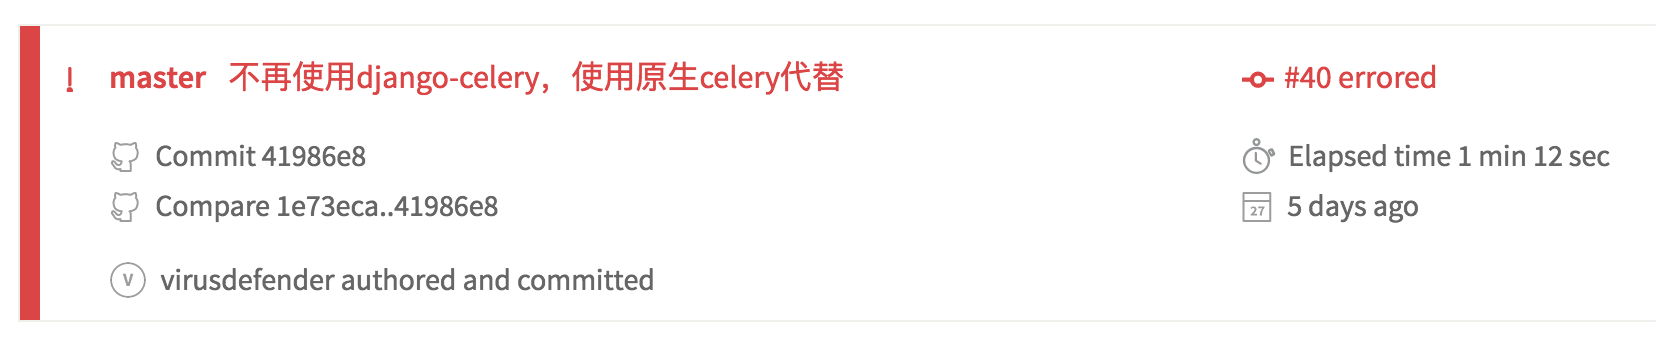
\includegraphics[width=0.9\textwidth]{ci-failed}
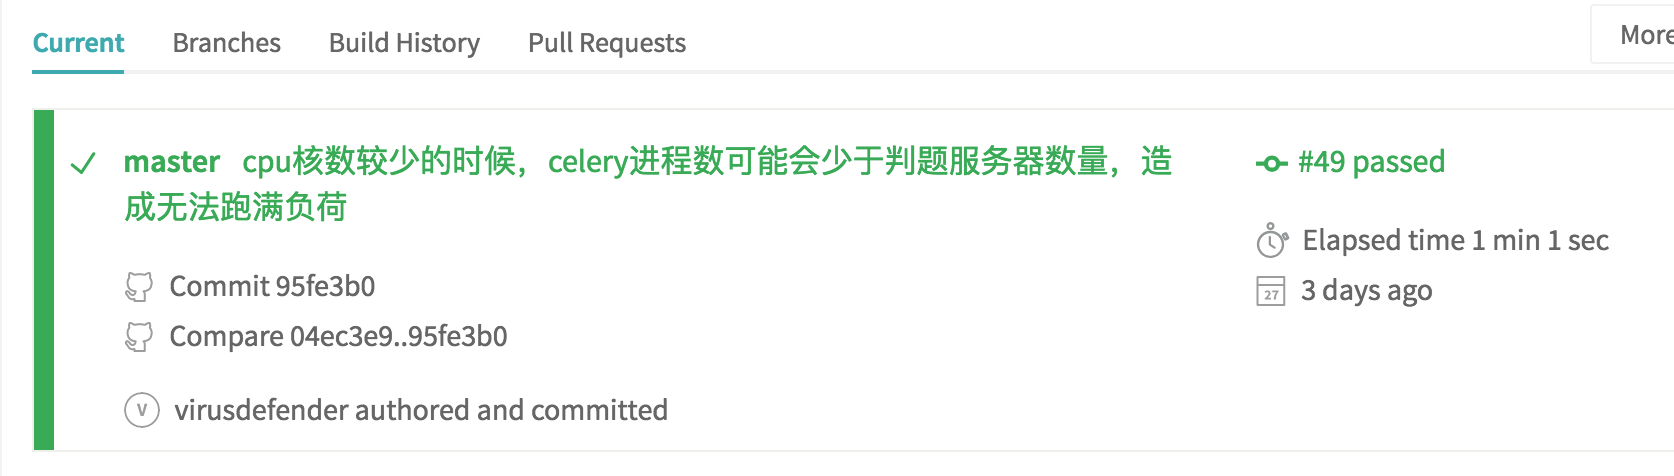
\includegraphics[width=0.9\textwidth]{ci-succeeded}
\caption{CI测试失败和通过的界面}
\end{figure}

如果测试通过,自动化部署的机器人就会拉取最新的代码,通过实现设定的脚本,自动化的更新测试环境,包括构建新的Docker镜像、应用数据库修改和重启Web Server等。

\subsection{使用Docker简化部署难度}
Docker是革命性的产品,通过镜像和容器大大简化了互联网产品的测试与部署难度。

本系统只需要通过Dockerfile全自动构建Docker镜像,然后简单配置docker-compose.yml文件,包括目录映射、部分环境变量和端口映射等,就可以直接运行。相比传统部署方式,隔离了服务器环境与系统的运行环境,大大降低了部署难度。

\texttt{Dockerfile}文件示例
\begin{verbatim}
FROM python:2.7
ENV PYTHONBUFFERED 1
RUN mkdir -p /code/log /code/test_case /code/upload
WORKDIR /code
ADD requirements.txt /code/
RUN pip install -r requirements.txt && rm /etc/apt/sources.list
ADD sources.list /etc/apt/
RUN curl -sL https://deb.nodesource.com/setup | bash -
RUN apt-get -y install nodejs
ADD gunicorn.conf /etc
ADD supervisord.conf /etc
ADD task_queue.conf /etc
EXPOSE 8080
CMD bash /code/dockerfiles/oj_web_server/run.sh
\end{verbatim}

\begin{figure}[H]
\centering
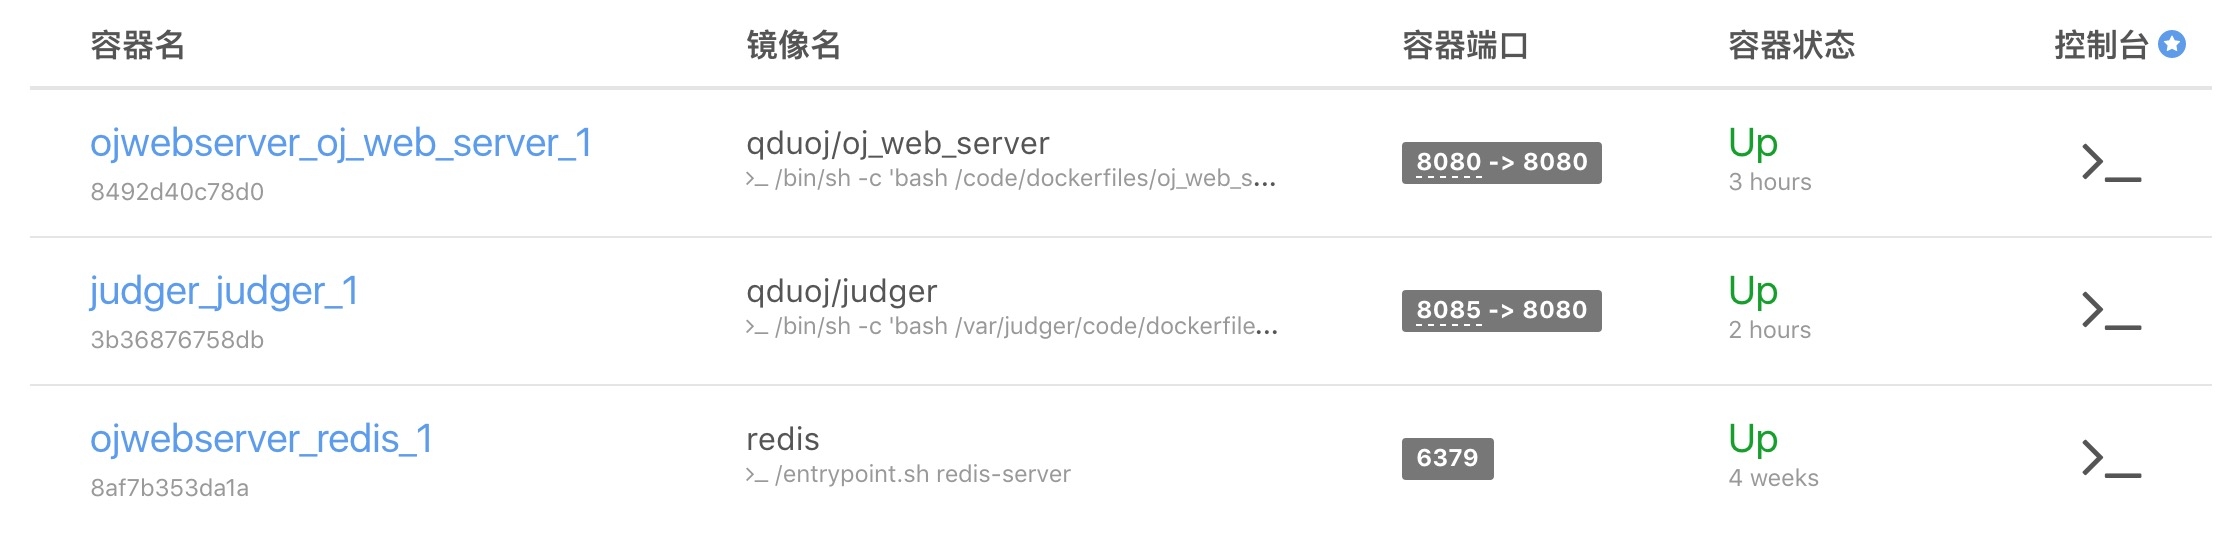
\includegraphics[width=\textwidth]{oj-docker}
\caption{OJ Docker运行情况}
\end{figure}